\documentclass{article}
\usepackage{amsmath}
\usepackage{amssymb}
\usepackage{graphicx}
\usepackage{float}
\usepackage{enumitem}
\usepackage{forest}

\begin{document}

\title{Homework 4}
\author{Manyara Bonface Baraka - mbaraka}
\date{\today}
\maketitle

\section{Distributed SGD}
SGD is an optimization method for training ml models by taking steps in the direction of the negative gradient using samples of the data. In distributed SGD, instead of doing
gradient computations on one machine:
\begin{itemize}
    \item We have \textbf{m worker nodes} that each of them compute gradient based on the local data.
    \item The gradients from all worker nodes are aggregated to update the model parameters.
    \item This process is repeated iteratively until convergence.
\end{itemize}
There are two major types of SGD strategies:
\begin{enumerate}
    \item \textbf{Synchronous SGD:} In this strategy, all worker nodes compute their gradients and send them to a central parameter server. The server aggregates the gradients and updates the model parameters. The updated parameters are then sent back to all worker nodes. This process ensures consistency but may suffer from delays caused by slower workers (stragglers).\\
    \[\text{Time per iteration = max of all X\_i}\]
    \item \textbf{Asynchronous SGD:} In this strategy, worker nodes compute gradients and send them to the parameter server independently. The server updates the model parameters as soon as it receives gradients from any worker. This approach is faster but may lead to stale updates, as some workers might use outdated model parameters.\\
    \[\text{Time per iteration = min of all X\_i}\]
\end{enumerate}


\clearpage
Consider that we have a system of $m$ worker nodes and a parameter server performing distributed SGD (stochastic gradient descent). In each iteration, every worker node receives the model from the parameter server, computes one gradient step of the objective function locally using its local data, and sends the gradient to the parameter server. The parameter server does the aggregation of gradients using either synchronous SGD or asynchronous SGD.

The gradient calculation time $X_i$ taken by each node $i$ follows the exponential distribution with rate $\lambda = 2$, which has the following probability density function (PDF):


\[
f_X(x) = 
\begin{cases} 
\lambda e^{-\lambda x}, & \text{if } x \geq 0 \\
0, & \text{else}
\end{cases}
\]



\begin{enumerate}
    \item[(a)] \textbf{Cumulative Distribution Function (CDF)}:
    What is the cumulative distribution function (CDF) of $f_X(x)$, i.e., $F_X(x)$?
    \subsubsection*{Solution}
    We are given that \(X \sim \text{Exponential}(\lambda = 2)\) and the pdf is:
    \[
    f_X(x)
    \begin{cases}
        2 e^{-2 x}, & \text{if } x \geq 0 \\
        0, & \text{else}
    \end{cases}
    \]

    The cumulative distribution function (CDF) is the integral of the PDF. For \(x \geq 0\), we compute:

    \[
    F_X(x) = \int_{0}^{x} f_X(t) \, dt = \int_{0}^{x} 2 e^{-2t} \, dt
    \]

    Intergration:

    \[
    F_X(x) = \left[ -e^{-2t} \right]_{0}^{x} = -e^{-2x} + e^{0} = 1 - e^{-2x}, \quad \text{for } x \geq 0
    \]

    For \(x < 0\), \(F_X(x) = 0\) since the PDF is 0 for \(x < 0\).

    Therefor, the CDF is:

    \[
    F_X(x) =
    \begin{cases}
    1 - e^{-2x}, & \text{if } x \geq 0 \\
    0, & \text{if } x < 0
    \end{cases}
    \]

    \item[(b)] \textbf{Maximum of $m$ Instances}:
    Define $X_{m:m}$ as the maximum of $m$ i.i.d. (independently and identically distributed) instances $X_1, \dots, X_m$ following the distribution $X$. What is the CDF of $X_{m:m}$, and what is the expected value $\mathbb{E}[X_{m:m}]$?
    \subsubsection*{Solution}
    \textbf{CDF of the Maximum $X_{m:m}$}\\

    The CDF of the maximum $X_{m:m}$ can be derived as follows:

    Let $F_X(x)$ be the CDF of a single instance $X$. The CDF of the maximum $X_{m:m}$ is given by:

    \[
    F_{X_{m:m}}(x) = P(X_{m:m} \leq x) = P(X_1 \leq x, X_2 \leq x, \dots, X_m \leq x)
    \]

    Since $X_1, X_2, \dots, X_m$ are i.i.d., we can write:

    \[
    F_{X_{m:m}}(x) = \prod_{i=1}^m P(X_i \leq x) = \left[F_X(x)\right]^m
    \]

    Substituting the CDF $F_X(x)$ from part (a):

    \[
    F_{X_{m:m}}(x) =
    \begin{cases}
    \left(1 - e^{-2x}\right)^m, & \text{if } x \geq 0 \\
    0, & \text{if } x < 0
    \end{cases}
    \]

    \textbf{Expected Value of $X_{m:m}$}

    The expected value $\mathbb{E}[X_{m:m}]$ of m i.i.d with rate \(\lambda\) is:

    \[
    \mathbb{E}[X_{m:m}] = \frac{1}{\lambda} \sum_{i = 1}^{m} \frac{1}{i}
    \]



    Since \(\lambda = 2\), therefore:

    \[
    \mathbb{E}[X_{m:m}] = \frac{1}{2} \sum_{i=1}^{m} \frac{1}{i}
    \]


    \item[(c)] \textbf{Minimum of $m$ Instances}:
    Define $X_{1:m}$ as the minimum of $m$ i.i.d. instances $X_1, \dots, X_m$ following the distribution $X$. What is the CDF of $X_{1:m}$, and what is the expected value $\mathbb{E}[X_{1:m}]$?
    \subsubsection*{Solution}

    \textbf{CDF of minimum $X_{1:m}$}

    The CDF of the minimum $X_{1:m}$ is derived by:

    If $F_X(x)$ is the CDF of a single instance $X$. The CDF of the minimum $X_{1:m}$ is:

    \[
    F_{X_{1:m}}(x) = P(X_{1:m} \leq x) = 1 - P(X_{1:m} > x) = 1 - P(X_1 > x, X_2 > x, \dots, X_m > x)
    \]

    Since $X_1, X_2, \dots, X_m$ are i.i.d., we write:

    \[
    F_{X_{1:m}}(x) = 1 - \prod_{i=1}^m P(X_i > x) = 1 - \left[1 - F_X(x)\right]^m
    \]

    Substituting the CDF $F_X(x)$ from part (a):

    \[F_{X_{1:m}}(x) = 1 - e^{-2mx} \]

    \[
    F_{X_{1:m}}(x) =
    \begin{cases}
    1 - e^{-2mx}, & \text{if } x \geq 0 \\
    0, & \text{if } x < 0
    \end{cases}
    \]

    \textbf{Expected Value of $X_{1:m}$}

    The expected value $\mathbb{E}[X_{1:m}]$ of the minimum of $m$ i.i.d. exponential random variables with rate $\lambda$ is:

    \[
    \mathbb{E}[X_{1:m}] = \frac{1}{m \lambda}
    \]

    Since $\lambda = 2$, we have:

    \[
    \mathbb{E}[X_{1:m}] = \frac{1}{2m}
    \]


    \item[(d)] \textbf{Simulation of Expected Runtime}:
    Simulate and compare the expected runtime per iteration of synchronous SGD and asynchronous SGD for different values of $m$. The time for each worker node to finish one gradient computation is exponentially distributed as given in part (a) with $\lambda = 2$, and it is i.i.d. across workers and iterations. Assume there is no communication delay.

    Simulate 5000 iterations of training using Python for different values of $m$ ranging from 1 to 20, and obtain the average runtime per iteration. Make a comparative plot of the average runtimes per iteration of synchronous and asynchronous SGD versus $m$. Explain the trends observed in the plot in 1-2 sentences. You may use packages inside \texttt{numpy.random} to draw random samples from the exponential distribution. Attach your plot and code in PDF format to the end of your homework.

    \subsubsection*{Solution}
    \begin{verbatim}
import numpy as np
import matplotlib.pyplot as plt

np.random.seed(42)

lambda_rate = 2
num_iter = 5000
m_values = range(1, 21)

sync_runtime = []
async_runtime = []

for m in m_values:
    sample = np.random.exponential(scale=1/lambda_rate, size=(num_iter, m))

    # Synchronous: max of each row
    sync_average = np.mean(np.max(sample, axis=1))
    sync_runtime.append(sync_average)

    # Assynchoronus: mean of each row
    async_average = np.mean(np.mean(sample, axis=1))
    async_runtime.append(async_average)

# Plotting
plt.figure(figsize=(10, 6))
plt.plot(m_values, sync_runtime, label='Synchronous SGD', marker='o')
plt.plot(m_values, async_runtime, label='Asynchronous SGD', marker='s')
plt.xlabel('Number of Worker Nodes (m)')
plt.ylabel('Average Runtime per Iteration')
plt.title('Synchronous vs Asynchronous SGD Runtimes')
plt.legend()
plt.grid(True)
plt.tight_layout()
plt.savefig("sgd_runtimes_plot.pdf")  # Save for submission
plt.show()        
    \end{verbatim}

    \textbf{Output}
    \begin{figure}[H]
        \centering
        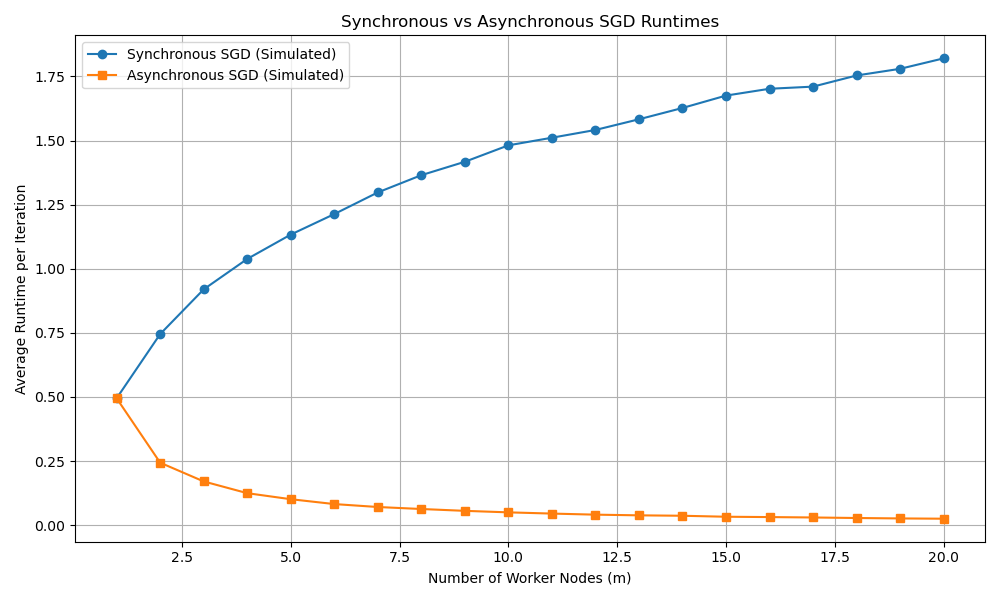
\includegraphics[width=1\textwidth]{SGD_simulation.png}
        % \caption{Comparison of Synchronous and Asynchronous SGD Runtimes}
        \label{fig:sgd_runtimes}
    \end{figure}

    \textbf{Trend Explained}\\
    \begin{itemize}
        \item The Sychronous SGD takes longer as m the number of workers increases because it waits for the slowest worker this leads to the max xomputation time grow with number of workers,
        \item The Assynchoronus SGD stabilizes with more workers this is beacuse the average of exponentially distributed varaibles converges quickly it becomes more efficeint as the number of workers increases.
    \end{itemize}

    \item[(e)] \textbf{Theoretical Expressions for Expected Runtimes}:
    Write down the theoretical expressions for the expected runtimes per iteration of synchronous and asynchronous SGD in terms of $m$ and $\lambda$. (Hint: You can use the expressions derived in parts (b) and (c)). On the figure generated in part (d), also plot the theoretical expected runtimes versus $m$. Check whether the theoretical and simulated values align.

    \subsubsection*{Solution}
    \textbf{Theoretical Expression for Synchronous}\\
    From part (b)
    \[\mathbb{E}[X_{m:m}] = \frac{1}{\lambda} \sum_{i=1}^{m} \frac{1}{i}\]

    \textbf{Theoretical Expression for Assynchoronus}\\
    Sincew the average of i.i.d exponential random variable with rate \(\lambda\) has the same mean therefore:
    \[\mathbb{E}[X_{1:m}] = \frac{1}{m \lambda}\]

    \begin{verbatim}
# Harmonic numbers for synchronous SGD
harmonic_numbers = np.array([np.sum(1 / np.arange(1, m + 1)) for m in m_values])
expected_sync = (1 / lambda_rate) * harmonic_numbers

# Expected runtime for asynchronous SGD is constant
expected_async = np.full_like(m_values, 1 / lambda_rate, dtype=np.float64)

# Plot: Simulated vs Theoretical runtimes
plt.figure(figsize=(10, 6))
plt.plot(m_values, sync_runtime, label='Simulated Sync SGD', marker='o')
plt.plot(m_values, async_runtime, label='Simulated Async SGD', marker='s')
plt.plot(m_values, expected_sync, label='Theoretical Sync SGD', linestyle='--', color='blue')
plt.plot(m_values, expected_async, label='Theoretical Async SGD', linestyle='--', color='orange')
plt.xlabel('Number of Worker Nodes (m)')
plt.ylabel('Average Runtime per Iteration')
plt.title('Simulated vs Theoretical SGD Runtimes')
plt.legend()
plt.grid(True)
plt.tight_layout()
plt.show()
    \end{verbatim}

    \begin{figure}[H]
        \centering
        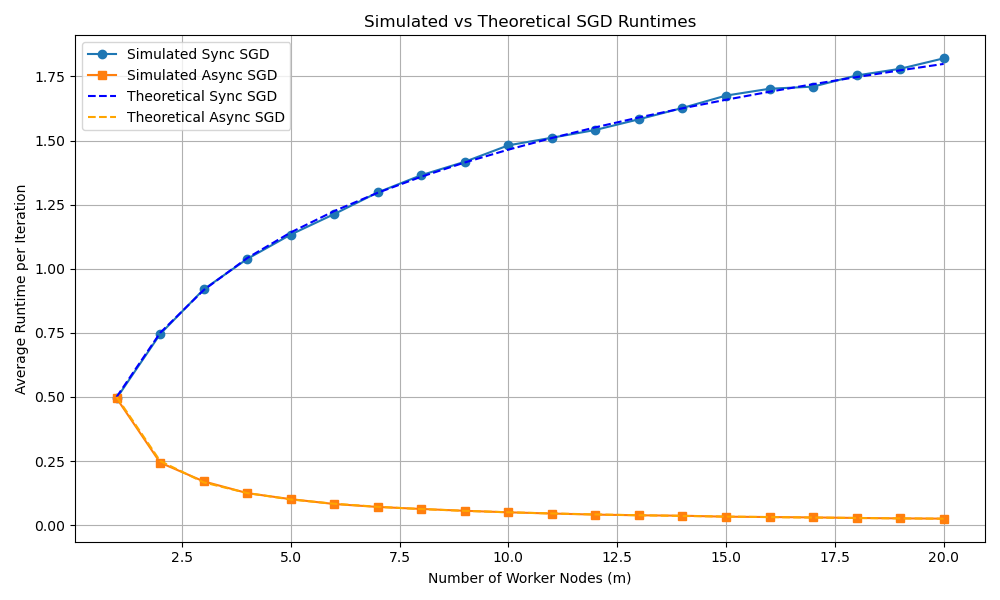
\includegraphics[width=0.85\textwidth]{SGD_simulation_theory.png}
        % \caption{Simulated vs Theoretical SGD Runtimes}
        \label{fig:sgd_simulation_theory}
    \end{figure}

    \textbf{Outcome Explained}\\
    The theoretical curves follows the simulated curves.
\end{enumerate}

\clearpage

\section{K-means}
K-means clustering is an unsupervised learning aligorithm that partititions a set of N datapoints to K clusters with an aim of minimizing the within-cluster variance or distortion
by assigning each data poitn to a cluster so that the sum of the squared distance between data points and theri correspondin clusters is minimized.





Given a set of data points $\{x_n\}_{n=1}^N$, k-means clustering minimizes the following distortion measure (also called the ``objective'' or ``clustering cost''):



\[
D = \sum_{n=1}^N \sum_{k=1}^K r_{nk} \|x_n - \mu_k\|_2^2
\]



where $\mu_k$ is the prototype of the $k$-th cluster and $r_{nk}$ is a binary indicator variable. If $x_n$ is assigned to the cluster $k$, $r_{nk}$ is 1, and otherwise $r_{nk}$ is 0. For each cluster, $\mu_k$ is the prototype representative for all the data points assigned to that cluster.

\begin{enumerate}
    \item [(a)] [10 points] In lecture, we stated but did not prove that $\mu_k$ is the mean of all points associated with the $k$-th cluster, thus motivating the name of the algorithm. You will now prove this statement. Assuming all $r_{nk}$ are known (i.e., assuming you know the cluster assignments of all $N$ data points), show that the objective $D$ is minimized when each $\mu_k$ is chosen as the mean of all data points assigned to cluster $k$, for any $k$. This justifies the iterative procedure of k-means.

    \subsubsection*{Solution}
    To minimize the objective \( D \), we differentiate it with respect to \(\mu_k\) and set the derivative to zero. The objective \( D \) is given by:

    \[
    D = \sum_{n=1}^N \sum_{k=1}^K r_{nk} \|x_n - \mu_k\|_2^2
    \]

    Expanding the squared norm:

    \[
    \|x_n - \mu_k\|_2^2 = (x_n - \mu_k)^\top (x_n - \mu_k) = x_n^\top x_n - 2 x_n^\top \mu_k + \mu_k^\top \mu_k
    \]

    Substituting this into \( D \):

    \[
    D = \sum_{n=1}^N \sum_{k=1}^K r_{nk} \left( x_n^\top x_n - 2 x_n^\top \mu_k + \mu_k^\top \mu_k \right)
    \]

    Rearranging terms:

    \[
    D = \sum_{n=1}^N \sum_{k=1}^K r_{nk} x_n^\top x_n - 2 \sum_{n=1}^N \sum_{k=1}^K r_{nk} x_n^\top \mu_k + \sum_{n=1}^N \sum_{k=1}^K r_{nk} \mu_k^\top \mu_k
    \]

    The first term does not depend on \(\mu_k\), so we can ignore it when minimizing \( D \). The remaining terms are:

    \[
    D = -2 \sum_{n=1}^N \sum_{k=1}^K r_{nk} x_n^\top \mu_k + \sum_{n=1}^N \sum_{k=1}^K r_{nk} \mu_k^\top \mu_k
    \]

    Now, differentiate \( D \) with respect to \(\mu_k\):

    \[
    \frac{\partial D}{\partial \mu_k} = -2 \sum_{n=1}^N r_{nk} x_n + 2 \mu_k \sum_{n=1}^N r_{nk}
    \]

    Set \(\frac{\partial D}{\partial \mu_k} = 0\) to find the optimal \(\mu_k\):

    \[
    -2 \sum_{n=1}^N r_{nk} x_n + 2 \mu_k \sum_{n=1}^N r_{nk} = 0
    \]

    Simplify:

    \[
    \mu_k \sum_{n=1}^N r_{nk} = \sum_{n=1}^N r_{nk} x_n
    \]

    Solve for \(\mu_k\):

    \[
    \mu_k = \frac{\sum_{n=1}^N r_{nk} x_n}{\sum_{n=1}^N r_{nk}}
    \]

    This shows that \(\mu_k\) is the mean of all points assigned to cluster \( k \), as required.



    \item [(b)] [10 points] As discussed in lecture, sometimes we wish to scale each feature in order to ensure that ``larger'' features do not dominate the clustering. Suppose that each data point $x_n$ is a $d$-dimensional feature vector and that we scale the $j$-th feature by a factor $w_j > 0$. Letting $W$ denote a $d \times d$ diagonal matrix with the $j$-th diagonal entry being $w_j, \, j = 1, 2, \ldots, d$, we can write our transformed features as $x' = Wx$.

    Suppose we fix the $r_{nk}$, i.e., we take the assignment of data points $x_n$ to clusters $k$ as given. Our goal is then to find the cluster centers $\mu_k$ that minimize the distortion measure:
    

\[
    D = \sum_{n=1}^N \sum_{k=1}^K r_{nk} \|Wx_n - \mu_k\|_2^2.
    \]



    Show that the cluster centers $\{\mu_k\}$ that do so are given by:
    

\[
    \mu_k = \left( \sum_{n=1}^N r_{nk} \right)^{-1} W \sum_{n=1}^N r_{nk} x_n.
    \]

    \subsubsection*{Solution}

    To minimize the distortion \( D \), we differentiate it with respect to \(\mu_k\) and set the derivative to zero. The distortion \( D \) is given by:

    \[
    D = \sum_{n=1}^N \sum_{k=1}^K r_{nk} \|Wx_n - \mu_k\|_2^2
    \]

    Expanding the squared norm:

    \[
    \|Wx_n - \mu_k\|_2^2 = (Wx_n - \mu_k)^\top (Wx_n - \mu_k) = x_n^\top W^\top W x_n - 2 x_n^\top W^\top \mu_k + \mu_k^\top \mu_k
    \]

    Substituting this into \( D \):

    \[
    D = \sum_{n=1}^N \sum_{k=1}^K r_{nk} \left( x_n^\top W^\top W x_n - 2 x_n^\top W^\top \mu_k + \mu_k^\top \mu_k \right)
    \]

    Rearranging terms:

    \[
    D = \sum_{n=1}^N \sum_{k=1}^K r_{nk} x_n^\top W^\top W x_n - 2 \sum_{n=1}^N \sum_{k=1}^K r_{nk} x_n^\top W^\top \mu_k + \sum_{n=1}^N \sum_{k=1}^K r_{nk} \mu_k^\top \mu_k
    \]

    The first term does not depend on \(\mu_k\), so we can ignore it when minimizing \( D \). The remaining terms are:

    \[
    D = -2 \sum_{n=1}^N \sum_{k=1}^K r_{nk} x_n^\top W^\top \mu_k + \sum_{n=1}^N \sum_{k=1}^K r_{nk} \mu_k^\top \mu_k
    \]

    Now, differentiate \( D \) with respect to \(\mu_k\):

    \[
    \frac{\partial D}{\partial \mu_k} = -2 \sum_{n=1}^N r_{nk} W x_n + 2 \mu_k \sum_{n=1}^N r_{nk}
    \]

    Set \(\frac{\partial D}{\partial \mu_k} = 0\) to find the optimal \(\mu_k\):

    \[
    -2 \sum_{n=1}^N r_{nk} W x_n + 2 \mu_k \sum_{n=1}^N r_{nk} = 0
    \]

    Simplify:

    \[
    \mu_k \sum_{n=1}^N r_{nk} = \sum_{n=1}^N r_{nk} W x_n
    \]

    Solve for \(\mu_k\):

    \[
    \mu_k = \left( \sum_{n=1}^N r_{nk} \right)^{-1} \sum_{n=1}^N r_{nk} W x_n
    \]

    Thus, the cluster centers \(\mu_k\) are given by:

    % \[
    % \mu_k = \left( \sum_{n=1}^N r_{nk} \right)^{-1} W \sum_{n=1}^N r_{nk} x_n
    % \]

    \[
    \mu_k = \frac{\sum_{n=1}^N r_{nk}Wx_n}{\sum_{n=1}^N r_{nk}}
    \]

\end{enumerate}



\clearpage

\section{3-Dimensional Principal Component Analysis}

In this problem, we will perform PCA on 3-dimensional data step by step. We are given three data points:


\[
x_1 = [0, -1, -2], \quad x_2 = [1, 1, 1], \quad x_3 = [2, 0, 1],
\]


and we want to find 2 principal components of the given data.

\begin{enumerate}
    \item[(a)] [8 points] First, find the covariance matrix $C_X = X^T X$ where:
    

\[
    X =
    \begin{bmatrix}
    x_1 - \bar{x} \\
    x_2 - \bar{x} \\
    x_3 - \bar{x}
    \end{bmatrix},
    \]


    and $\bar{x} = \frac{1}{3}(x_1 + x_2 + x_3)$ is the mean of the data samples. Then, find the eigenvalues and the corresponding eigenvectors of $C_X$. Feel free to use any numerical analysis program such as \texttt{numpy}, e.g., \texttt{numpy.linalg.eig} can be useful. However, you should explain what you inputted into this program.

    \subsubsection*{Solution}

    First, calculate the mean of the data samples:

    \[
    \bar{x} = \frac{1}{3}(x_1 + x_2 + x_3) = \frac{1}{3} \left([0, -1, -2] + [1, 1, 1] + [2, 0, 1]\right) = [1, 0, 0].
    \]

    Next, subtract the mean from each data point to form the matrix \( X \):

    \[
    X =
    \begin{bmatrix}
    x_1 - \bar{x} \\
    x_2 - \bar{x} \\
    x_3 - \bar{x}
    \end{bmatrix}
    =
    \begin{bmatrix}
    [0, -1, -2] - [1, 0, 0] \\
    [1, 1, 1] - [1, 0, 0] \\
    [2, 0, 1] - [1, 0, 0]
    \end{bmatrix}
    =
    \begin{bmatrix}
    -1 & -1 & -2 \\
    0 & 1 & 1 \\
    1 & 0 & 1
    \end{bmatrix}.
    \]

    The covariance matrix \( C_X \) is given by:

    \[
    C_X = X^\top X.
    \]

    Compute \( X^\top \):

    \[
    X^\top =
    \begin{bmatrix}
    -1 & 0 & 1 \\
    -1 & 1 & 0 \\
    -2 & 1 & 1
    \end{bmatrix}.
    \]

    Now, calculate \( C_X \):

    \[
    C_X = X^\top X =
    \begin{bmatrix}
    -1 & 0 & 1 \\
    -1 & 1 & 0 \\
    -2 & 1 & 1
    \end{bmatrix}
    \begin{bmatrix}
    -1 & -1 & -2 \\
    0 & 1 & 1 \\
    1 & 0 & 1
    \end{bmatrix}.
    \]

    Matrix multiplication:

    \[
    C_X =
    \begin{bmatrix}
    2 & 1 & 3 \\
    1 & 2 & 3 \\
    3 & 3 & 6
    \end{bmatrix}.
    \]

    Found the Eigenvalues and eigenvectors:
    \begin{verbatim}
import numpy as np

Cx = np.array([
    [2, 1, 3],
    [1, 2, 3],
    [3, 3, 6]
])

eigvals, eigvecs = np.linalg.eig(Cx)
print("EigenValues:", eigvals)
print("Eigen Vectors", eigvecs)
    \end{verbatim}
    Eigenvalues:
     \[
     \lambda_1 = 9.000, \quad \lambda_2 = 1.000, \quad \lambda_3 = 1.054 \times 10^{-16}.
     \]

     Eigenvectors (corresponding to \( \lambda_1, \lambda_2, \lambda_3 \)):
     \[
     u_1 = \begin{bmatrix} -0.408 \\ -0.408 \\ -0.816 \end{bmatrix}, \quad
     u_2 = \begin{bmatrix} -0.707 \\ 0.707 \\ 0.000 \end{bmatrix}, \quad
     u_3 = \begin{bmatrix} -0.577 \\ -0.577 \\ 0.577 \end{bmatrix}.
     \]

    \item[(b)] [4 points] Using the result above, find the first two principal components of the given data.
    \subsubsection*{Solution}
    From part a above, to find the first top 2 princible component we select the top 2 eigenvectors corresponding to the top eigenvalues. 
    \[
    \lambda_1 = 9.000, \quad \lambda_2 = 1.000, \quad 
    \]

    The eigenvectors corresponding to \(\lambda_1\) and \(\lambda_2\) are:

    \[
    u_1 = \begin{bmatrix} -0.408 \\ -0.408 \\ -0.816 \end{bmatrix}, \quad
    u_2 = \begin{bmatrix} -0.707 \\ 0.707 \\ 0.000 \end{bmatrix}.
    \]

    Therefore, the first two principal components are:

    \[
    u_1 = \begin{bmatrix} -0.408 \\ -0.408 \\ -0.816 \end{bmatrix}, \quad
    u_2 = \begin{bmatrix} -0.707 \\ 0.707 \\ 0.000 \end{bmatrix}.
    \]


    \item[(c)] [8 points] Now we want to represent the data $x_1, \cdots, x_3$ using a 2-dimensional subspace instead of a 3-dimensional one. PCA gives us the 2-D plane which minimizes the difference between the original data and the data projected to the 2-dimensional plane. In other words, $x_i$ can be approximated as:
    

\[
    \hat{x}_i = a_{i1}u_1 + a_{i2}u_2 + \bar{x},
    \]


    where $u_1$ and $u_2$ are the principal components we found in 3.(b). Figure 1 gives an example of what this might look like.

    Find $a_{i1}, a_{i2}$ for $i = 1, 2, 3$. Then, find the $\hat{x}_i$'s and the difference between $\hat{x}_i$ and $x_i$, i.e., $\|\hat{x}_i - x_i\|_2$ for $i = 1, 2, 3$. (Again, feel free to use any numerical analysis program to get the final answer, but show your calculation process.)

    \subsubsection*{Solution}

    Have defined the calculation steps in the comments.
    \begin{verbatim}
import numpy as np

# Original data
data = np.array([
    [0, -1, -2],
    [1,  1,  1],
    [2,  0,  1]
])

# Compute the mean
mean_vector = np.mean(data, axis=0)

# Define the Center the data
X_centered = data - mean_vector

# Given covariance matrix
Cx = np.array([
    [2, 1, 3],
    [1, 2, 3],
    [3, 3, 6]
])

# Eigen decomposition
eigvals, eigvecs = np.linalg.eig(Cx)
print("Eigenvalues:", eigvals)
print("Eigenvectors:\n", eigvecs)

# Furst 2 principal components (eigenvectors)
U = eigvecs[:, :2]  # Take first two columns (PC1 and PC2)

# Project centered data onto 2D principal subspace
A = X_centered @ U

# Reconstructing the data using the top 2 PCs
X_reconstructed = A @ U.T + mean_vector

# Computing reconstruction errors
errors = np.sum((data - X_reconstructed)**2, axis=1)

# Display results
print("\nProjection coefficients (a_i):\n", A)
print("\nReconstructed data (x_i_hat):\n", X_reconstructed)
print("\nReconstruction errors ||x_i - x_i_hat||^2:\n", errors)

    \end{verbatim}

    \textbf{Output:}
    \textbf{Projection coefficients ($a_i$):}
    \[
    \begin{bmatrix}
        2.44948974 \times 10^0 & 2.62480955 \times 10^{-17} \\
     -1.22474487 \times 10^0 & 7.07106781 \times 10^{-1} \\
     -1.22474487 \times 10^0 & -7.07106781 \times 10^{-1}
    \end{bmatrix}
    \]

    \textbf{Reconstructed data ($\hat{x}_i$):}
    \[
    \begin{bmatrix}
        0.00000000 \times 10^0 & -1.00000000 \times 10^0 & -2.00000000 \times 10^0 \\
        1.00000000 \times 10^0 &  1.00000000 \times 10^0 &  1.00000000 \times 10^0 \\
        2.00000000 \times 10^0 &  1.66533454 \times 10^{-16} &  1.00000000 \times 10^0
    \end{bmatrix}
    \]

    \textbf{Reconstruction errors $\|\hat{x}_i - x_i\|_2^2$:}
    \[
    \begin{bmatrix}
        1.97215226 \times 10^{-31} \\
        2.58844985 \times 10^{-31} \\
        2.77333912 \times 10^{-32}
    \end{bmatrix}
    \]
    
\end{enumerate}


\clearpage

\section{Clustering Human Activity using Inertial Sensors Data}

\subsection{Import Data and Plotting}
Visual of PCA wiht different colors with respective activity labels

\begin{figure}[H]
    \centering
    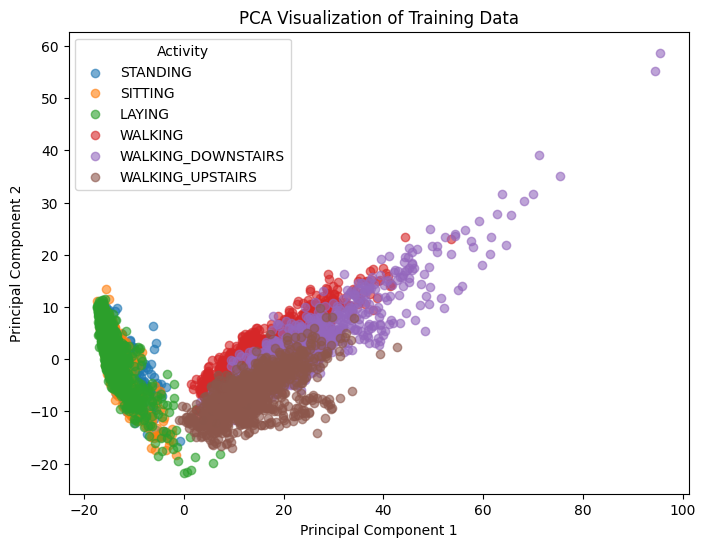
\includegraphics[width=1\textwidth]{image.png}
    % \caption{PCA visualization of human activity clustering with different colors representing activity labels.}
    \label{fig:human_activity_pca}
\end{figure}

\clearpage

\subsection{Choosing the optimal Number of Clusters}
\begin{enumerate}
    \item [(a)] \textbf{Elbow Method}
    \begin{figure}[H]
        \centering
        \begin{minipage}{0.5\textwidth}
            \centering
            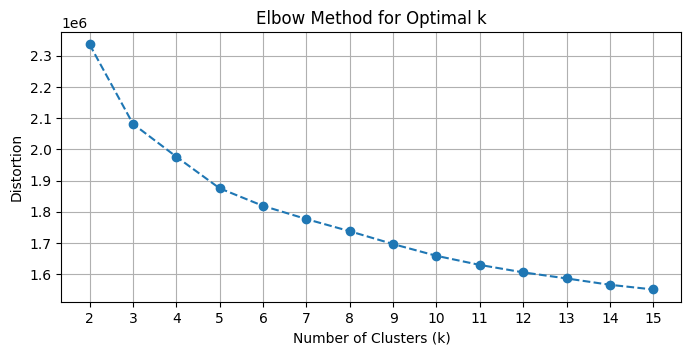
\includegraphics[width=\textwidth]{elbow_meth.png}
            % \caption{Elbow method for determining the optimal number of clusters.}
            \label{fig:elbow_method}
        \end{minipage}
        \hfill
        \begin{minipage}{0.45\textwidth}
            \centering
            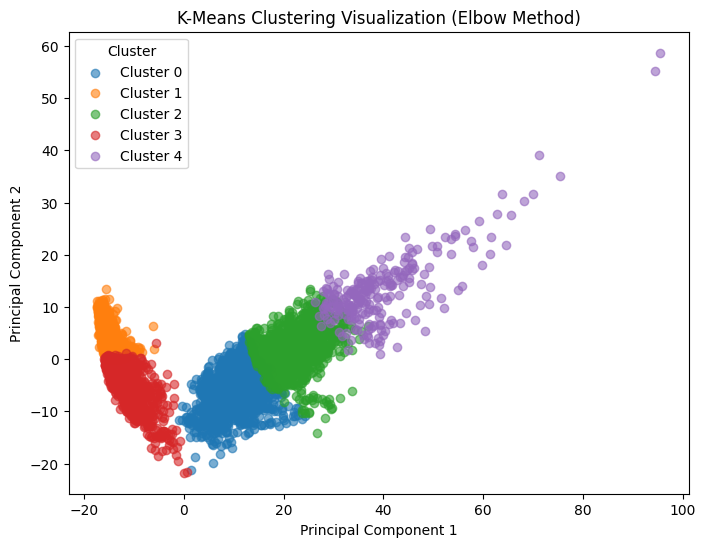
\includegraphics[width=\textwidth]{elbow_graph.png}
            % \caption{Elbow graph for visualizing cluster selection.}
            \label{fig:elbow_graph}
        \end{minipage}
    \end{figure}
    - The optimal number of cluser is 6.\\
    - Distortion measures the sum of the squared distance between the  data points and the assigned clustes this means an increase in the clusters leads to the 
    decrease of the the distortion. This is mainly because increaseing clusters allows the centroing to better fit the data which reduces the distance between points 
    and their nearest centroid. However, as K becomes large the distortion the decreasing rate also diminishes  which leads to the elbow point where addding more clustersprovides the diminishing returns in reducing distortion.

    \item [(b)] \textbf{Adjusted Rand Index}
    \begin{figure}[H]
        \centering
        \begin{minipage}{0.5\textwidth}
            \centering
            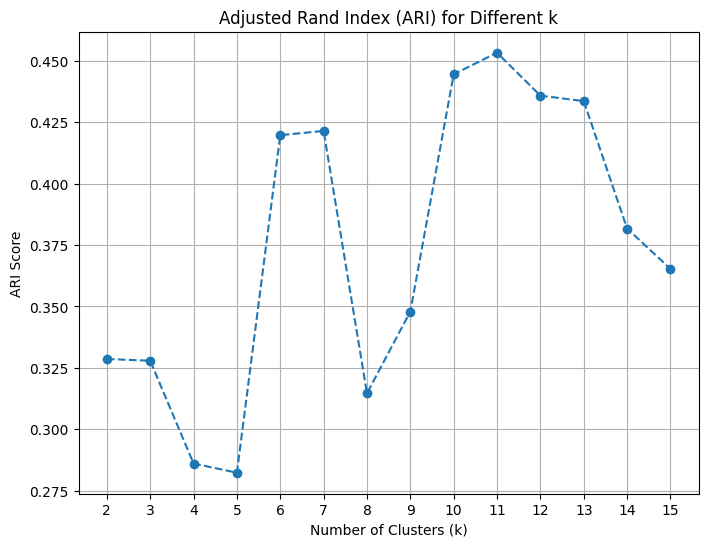
\includegraphics[width=\textwidth]{Ari_plot.png}
            % \caption{Adjusted Rand Index plot for clustering evaluation.}
            \label{fig:ari_plot}
        \end{minipage}
        \hfill
        \begin{minipage}{0.45\textwidth}
            \centering
            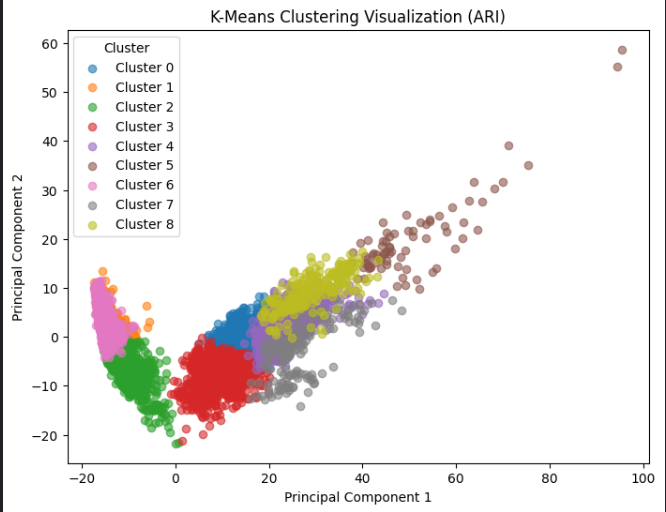
\includegraphics[width=\textwidth]{Ari_graph.png}
            % \caption{Adjusted Rand Index graph for visualizing clustering performance.}
            \label{fig:ari_graph}
        \end{minipage}
    \end{figure}
    - The optimal was 11.\\
    - ARI measures the similarity between clustering results and the ground truth labels. As the number of clusters increase the followng trend is observeds.
    \begin{itemize}
        \item Plateau: Beyond the optimal K, the Ari scrore declines as the clusters become too granular, this leads reduction of alignment with the ground truth.
        \item Fluctuations: As K increases, the ARI fluctuares due to creation of more clustres that do not correspond well to the true data distributions or overfitting.
    \end{itemize}
\end{enumerate}

\subsection{Prototype Selection using K-means clustering}
\begin{enumerate}
    \item [(a)] \textbf{Random Selection} : Average Accuracy with Random Selection over 10 repetitions: 0.9223.
    \item [(b)] \textbf{Using K-means clustering by Class} : Accuracy with K-means Selection: 0.9057
\end{enumerate}

\subsubsection*{Comparizon of the Random selection and the K-meands clusering by class model Accuracy}
The Random prototype selection had a higher Accuracy of 92.23\% compared to the K-means clustering that had 90.57\%, this could be becaue Random seelction relies on randomly selected prototypes that
may capture diverse sample from each class while K-means clustering selects the prototype based on clusters that ensure that the selected samples are representative of the cluser centroids 
however, this may miss some outlier or diverse samples. And since the later focuess more on centroirds rather than capturing the full variablity of the data this may be the reason of the less performance of the models
compared to the reandom selection model.

\end{document}